%----------------------------------------------------------------------------------------------------
\section{Analysis}

The analysis method is similar to the previously published ones~\cite{epl101-el,prl111}, each diagonal is analysed
separately. However, a different normalisation
approach is used (Section~\ref{sec:normalisation}), making all 
$t$-independent scaling factors irrelevant.



%----------------------------------------------------------------------------------------------------

\subsection{Event Reconstruction}

Event kinematics are determined from track hits in the RPs after proper 
alignment (see Section~\ref{sec:alignment}), using the LHC optics 
(see Section~\ref{sec:optics}).

%------------------------------

\subsubsection{Kinematics Determination}
\label{sec:kinematics}

The scattering angles and vertex position are first determined for each proton (i.e.~from each arm) separately by inverting the proton transport Eq.~(\ref{eq:prot trans}). The following formulae optimise the robustness against optics imperfections:
\begin{equation}
\label{eq:kin 1a}
	\begin{aligned}
		\theta_x^* &= {v_x^{\rm N} x^{\rm F} - v_x^{\rm F} x^{\rm N}\over v_x^{\rm N} L_x^{\rm F} - v_x^{\rm F} L_x^{\rm N}}\ ,\qquad
		\theta_y^* = {1\over 2} \left( {y^{\rm N}\over L_y^{\rm N}} + {y^{\rm F}\over L_y^{\rm F}} \right)\ ,\\
		x^* &= {L_x^{\rm N} x^{\rm F} - L_x^{\rm F} x^{\rm N}\over L_x^{\rm N} v_x^{\rm F} - L_x^{\rm F} v_x^{\rm N}}\ , \\
	\end{aligned}
\end{equation}
where the N and F superscripts refer to the near and far units, $x$ and $y$ to horizontal and vertical track hits and $v$ and $L$ stand for the magnification and effective length optical functions. This one-arm reconstruction is used for tagging elastic events, where the left and right arm protons are compared.

Once an event is selected, the information from both arms can be merged yielding better angular resolution:
\begin{equation}
\label{eq:kin 2a}
\theta_x^* = {\theta_x^{*\rm L} + \theta_x^{*\rm R} \over 2}\ ,\quad \theta_y^* = {\theta_y^{*\rm L} + \theta_y^{*\rm R} \over 2}\ ,
\end{equation}
where the L (R) superscript refers to the left (right) arm.

Eventually, the full scattering angle, $\theta^*$, and four-momentum transfer squared, $t$, are calculated as

\begin{equation}
\label{eq:th t}
\theta^* = \sqrt{{\theta_x^*}^2 + {\theta_y^*}^2}\ ,\quad t = - p^2 ({\theta_x^*}^2 + {\theta_y^*}^2)\ ,
\end{equation}
where $p$ denotes the beam momentum.

%------------------------------

\subsubsection{Alignment}
\label{sec:alignment}

The standard three-step procedure \cite{totem-ijmp} has been applied: beam-based alignment prior to the run (as for LHC collimators) followed by two off-line methods: track-based alignment (for relative positions among RPs) and alignment with elastic events (for absolute position with respect to the beam). The final uncertainties per unit (common for top and bottom RPs) are: $2\un{\mu m}$ (horizontal shift), $100\un{\mu m}$ (vertical shift) and $0.2\un{mrad}$ (rotation about the beam axis). Propagated to the scattering angles, Eq.~(\ref{eq:kin 2a}), the shifts lead to uncertainties of $0.8\un{\mu rad}$ (horizontal) and $0.2\un{\mu rad}$ (vertical). The error of the RP rotations would bias the reconstructed $\theta_x^*$ by a term proportional to $\theta_y^*$, with the proportionality constant having a standard deviation of $0.02$. \todo{effect of such bias}


%------------------------------

\subsubsection{Optics}
\label{sec:optics}

In order to reduce the impact of imperfect optics knowledge, the optics matching technique \cite{totem-optics} has been applied. The residual imperfections induce an error in the reconstructed scattering angle proportional to the angle. For the two-arm reconstruction, Eq.~(\ref{eq:kin 2a}), the proportionality constants have uncertainties of $0.21\un{\%}$ (horizontal) and $0.25\un{\%}$ (vertical), including the effects of magnet harmonics.

\iffalse
% original text
In order to reduce errors due to imperfect optics knowledge, the optics matching technique \cite{totem-optics} has been applied. The 
corrections have the form of factors scaling the scattering angles
For the two-arm reconstruction, Eq.~(\ref{eq:kin 2a}), the factors have uncertainties of $0.21\un{\%}$ (horizontal) and $0.25\un{\%}$ (vertical), including the effects of magnet harmonics.
\fi

% double-arm; before matching $0.48\un{\%}$ (hor), $0.90\un{\%}$


%------------------------------

\subsubsection{Resolution}
\label{sec:resolution}

Statistical fluctuations in the reconstructed scattering angles are caused by 
the beam divergence and, in the horizontal projection (due to small $L_x$), 
also by the sensor resolution. Good descriptions of these effects
are essential for several corrections discussed below.

The angular resolution is studied through differences $\theta_{x,y}^{*R} - \theta_{x,y}^{*L}$. Since in good approximation the fluctuations are independent in each arm, the distribution of the difference is just twice wider than the fluctuation of angles in Eq.~(\ref{eq:kin 2a}). Generally, the distributions are well Gaussian, the small non-Gaussianity is decreasing with time. The resolutions were found to deteriorate with time: for the two-arm $\theta_y^*$ it evolved from initially $1.6$ to $1.7\un{\mu rad}$ at the end of the run. For $\theta_x^*$, the resolution decreased from $4.6$ to $4.8\un{\mu rad}$ (for the diagonal 45 bottom -- 56 top) and from $4.3$ to $4.4\un{\mu rad}$ (45 top -- 56 bottom).

Measurements of beam emittances \todo{citation ??} show that the vertical beam divergences of the two beams are equal with a tolerance of about $15\un{\%}$. Exploiting this equality, one can de-convolute the distribution of $\theta_y^{*R} - \theta_y^{*L}$ in order to obtain the beam-divergence distribution, used e.g.~for acceptance corrections (see Section~\ref{sec:acc corr}).

\todo{standard emittance growth ??}


\iffalse
The resolution in $\theta_y^*$ decreased from $1.6$ to $1.7\un{\mu rad}$ from the beginning to the end of the fill (DS3+DS4), for $\theta_x^*$ from $4.6$ to $4.8\un{\mu rad}$ (45b -- 56t) and from $4.3$ to $4.4\un{\mu rad}$ (45t -- 56b). In fact, just means over all bunches -- in analysis bunches treated independently. Comparing x and y, the contribution from the RP spatial resolution is evident. A cross check, horizontal beam div. from vertex distribution (sigma 145 to 185 urad, diagonal independent) % 2.3 to 2.9 urad
, the sensor contribution (2-arm) is $4.3$ (45b) and $4.0$ urad (45t), time independent. With the same method, not only RMS, but also shape. Generally, gaussian-like, with non-gaussianity decreasing with time. Non-gaussianinty taken accounted in systematic uncertainties. The original assumption of identical resolutions in both arms can be verified by checking the beam emittances. They give beam divergences compatible with our observations and indicate that a possible left-right imbalance could be of order $15\un{\%}$, which is used for uncertainty estimation.
\fi

\begin{figure}
\begin{center}
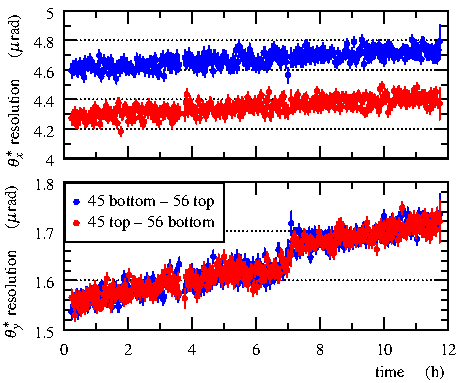
\includegraphics{fig/resolutions_vs_time.pdf}
\vskip-4mm
\caption{%
\todo{caption}. Double-arm angular resolution as a function of time (from the beginning of the first data-taking day). The step in $\theta_y^*$ resolution around $26.5\un{h}$ is due to inclusion of another bunch with a larger vertical emittance.
}
\label{fig:resolutions}
\end{center}
\end{figure}


\begin{figure}
\begin{center}
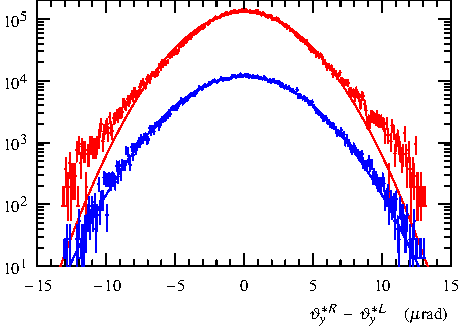
\includegraphics{fig/beam_divergence_fits.pdf}
\vskip-4mm
\caption{%
\todo{caption}. Diagonal 45 bottom - 56 top. Red: data between $20$ and $21\un{h}$. Blue: data between $30$ and $31\un{h}$, scaled by $0.1$. The solid lines represent single-Gaussian fits.
}
\label{fig:beam divergence}
\end{center}
\end{figure}


%----------------------------------------------------------------------------------------------------

\subsection{Differential Cross-Section}
\label{sec:diff cs}

For a given $t$ bin, the differential cross-section is evaluated by selecting and counting elastic events:
\begin{equation}
{\d\sigma\over \d t}(\hbox{bin}) =
	{\cal N}\, {\cal U}({\rm bin})\, {\cal B}\ 
	{\sum\limits_{t \in \hbox{bin}} {\cal A}(\theta^*, \theta_y^*)\, {\cal E}(\theta_y^*)\over \Delta t}\ ,
\end{equation}
where $\Delta t$ is the width of the bin, ${\cal N}$ is a normalisation factor, 
and the other symbols stand for various correction factors:
${\cal U}$ for unfolding of resolution effects, ${\cal B}$ for background subtraction, ${\cal A}$ for acceptance correction and ${\cal E}$ for detection and reconstruction efficiency.

%------------------------------

\subsubsection{Event Tagging}
\label{sec:tagging}

The cuts used to select elastic events are summarised in Table \ref{tab:cuts}. Cuts 1 and 2 require the reconstructed-track collinearity between the left and right arm. Cuts 3 and 4 control the elasticity -- if a proton loses momentum, the vertical position-angle correlation at the RPs is lost. Cut 5 ensures that the two protons come from the same vertex (horizontally). The correlation plots corresponding to these cuts are shown in Figure~\ref{fig:cuts}.

Monte-Carlo simulation suggests that applying all the five cuts at $3\un{\sigma}$ level would lead to a loss of about $2\un{\%}$ of elastic events. Setting the thresholds to $4\un{\sigma}$ yields a tolerable loss of about $0.07\un{\%}$ and therefore the cuts are applied at the $4\un{\sigma}$ level.
% 2sigma: 76%, 3sigma: 98.02%, 4sigma: 99.93%, 5sigma: 99.999%

The tagging efficiency is studied experimentally by applying the cuts also at the $5\un{\sigma}$ level. This selection yields about $0.5\un{\%}$ more events in every $t$ bin -- thus the inefficiency is irrelevant for the presented analysis.


\begin{table}
\caption{The elastic selection cuts. The superscripts R and L refer to the right and left arm, N and F correspond to the near and far units, respectively. The constant $\alpha = L_y^{\rm F} / L_y^{\rm N} - 1 \approx 0.11$. The right-most column gives a typical RMS of the cut distribution.
}
\label{tab:cuts}
\begin{center}
\vskip-3mm
\begin{tabular}{ccc}\hline\hline
number & cut & RMS ($\equiv 1\sigma$)\cr\hline
1 & $\theta_x^{*\rm R} - \theta_x^{*\rm L}$				& $9.5\un{\mu rad}$	\cr
2 & $\theta_y^{*\rm R} - \theta_y^{*\rm L}$				& $3.3\un{\mu rad}$	\cr
3 & $\alpha\,y^{\rm R,N} - (y^{\rm R,F} - y^{\rm R,N})$	& $18\un{\mu m}$	\cr
4 & $\alpha\,y^{\rm L,N} - (y^{\rm L,F} - y^{\rm L,N})$	& $18\un{\mu m}$	\cr
5 & $x^{*\rm R} - x^{*\rm L}$							& $8.5\un{\mu m}$ 	\cr\hline\hline
\end{tabular}
\end{center}
\end{table}

\begin{figure*}
\begin{center}
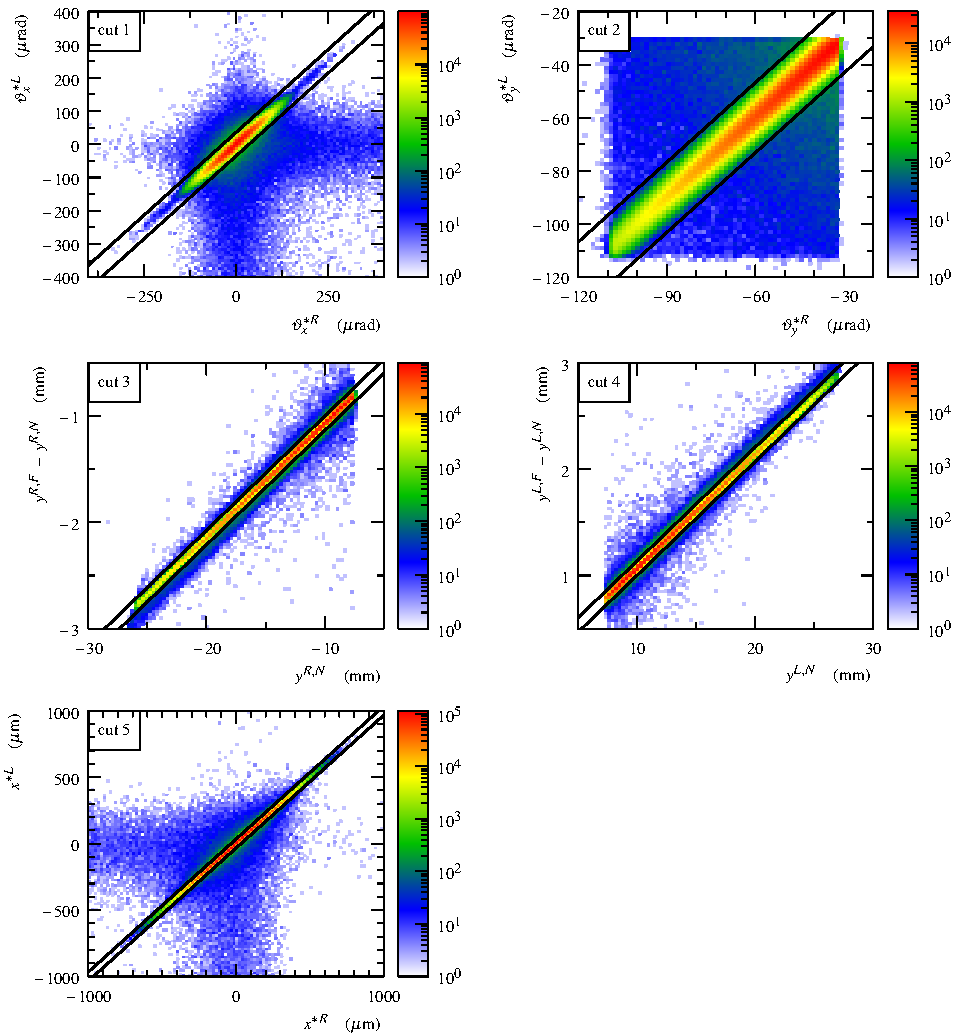
\includegraphics{fig/cuts.pdf}
\caption{%
Correlation plots for the selection cuts summarised in Table~\ref{tab:cuts}, using all events with diagonal topology 45 top -- 56 bottom. The black solid lines delimit the signal ($\pm 4\un{\sigma}$) region.
}
\label{fig:cuts}
\end{center}
\end{figure*}


%------------------------------

\subsubsection{Background}
\label{sec:background}

Figure~\ref{fig:background} shows distributions of several discriminators from Table~\ref{tab:cuts} under various cut combinations. While the central part (signal) remains essentially constant, the tails (background) are strongly suppressed with increasing number of cuts applied. Interpolating the background smoothly into the signal region (see the dotted lines in the figure) yields a background estimate of $1 - {\cal B} < 10^{-4}$, independent of whether discriminator 1, 2 or 5 is used.
% anyway irrelevant due to the normalisation approach

\todo{what could the background be}


\begin{figure}
\begin{center}
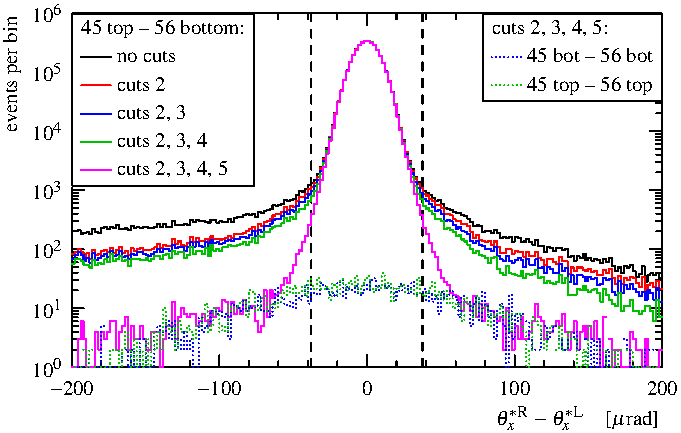
\includegraphics{fig/cut_distributions.pdf}
\caption{%
\todo{just an example}
Right-left differences of the reconstructed scattering angles ($\theta_x^*$, $\theta_y^*$) and horizontal vertex position ($x^*$) under various combinations of the selection cuts, using all events with diagonal topology 45 top -- 56 bottom. The cut numbers in the legend correspond to Table~\ref{tab:cuts}. The vertical dashed lines represent the boundaries of the signal region ($\pm 4\un{\sigma}$ of the central peak). The dotted lines give a smooth interpolation (Gaussian fit) of the background observed in the distribution tails.
}
\label{fig:background}
\end{center}
\end{figure}

%-------------------------

\subsubsection{Acceptance Correction}
\label{sec:acc corr}

Two detection limitations have been identified: detector coverage (mostly at the edge facing the beam, i.e. relevant for small $|\theta_y^*|$) and LHC apertures ($|\theta_y^*| \sim 100\un{\mu rad}$). The acceptance correction includes two contributions -- a geometrical correction ${\cal A}_{\rm geom}$ reflecting the fraction of the phase space within the acceptance and a component ${\cal A}_{\rm fluct}$ correcting for fluctuations around the acceptance limitations \todo{limitations cuts in y, thus function of $\theta_y^*$}:
\begin{equation}
{\cal A}(\theta^*, \theta_y^*) = {\cal A}_{\rm geom}(\theta^*)\ {\cal A}_{\rm fluct}(\theta_y^*)\ .
\end{equation}

The calculation of the geometrical correction ${\cal A}_{\rm geom}$ is based on the azimuthal symmetry of elastic scattering, experimentally verified for the data within acceptance. The correction is given by the inverse of the fraction of a circle with radius $\theta^*$ falling into the acceptance region in the ($\theta_x^*$, $\theta_y^*$) space. The value of the correction drops rapidly from $5$ at the lowest $|t|$ to about $2.5$ at $|t| = 0.15\un{GeV^2}$ and then increases again to about $4$ at $|t| = 0.2\un{GeV^2}$.

The correction ${\cal A}_{\rm fluct}$ is calculated analytically from the probability that any of the two elastic protons is pushed outside the acceptance due to the beam divergence. The beam divergence distribution is modelled as Gaussian with spread determined by the method described in Section~\ref{sec:resolution}. This correction contribution is only sizeable close to the acceptance limitations but remains below $1.5$. The uncertainties are related to the resolution parameters (vertical beam divergence, left-right asymmetry and non-Gaussian shape), and all stay below $0.1\un{\%}$.


\iffalse
\begin{equation}
\label{acceptance}
{\cal A_{\rm sm}}(\theta_y^*)^{-1} = {1\over 2} \left(
	\mathop{\rm Erf} {\min(\theta_y^{*,R,max} - |\theta_y^*|, |\theta_y^*| - \theta_y^{*,L,min})\over \sigma^{1a}_{\theta_y^*}}
	- \mathop{\rm Erf} {\max(\theta_y^{*,R,min} - |\theta_y^*|, |\theta_y^*| - \theta_y^{*,L,max})\over \sigma^{1a}_{\theta_y^*}}
\right)
\end{equation}

\begin{equation}
\label{acceptance}
{\cal A_{\phi}}(\theta_y^*) = {
	2\pi\over 
	\hbox{arc length with $\theta_y^*$ between } \max(\theta_y^{*,L,min}, \theta_y^{*,R,min}) \hbox{ and } \min(\theta_y^{*,L,max}, \theta_y^{*,R,max})
}
\end{equation}
\fi


\begin{figure}
\begin{center}
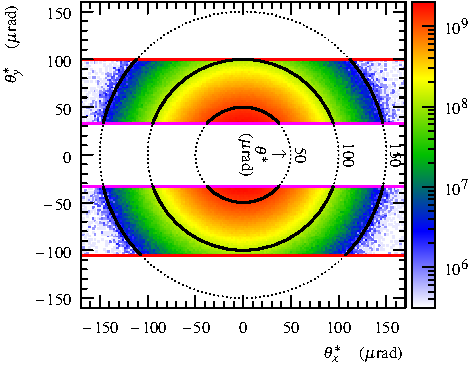
\includegraphics{fig/acc_corr_phi_lab.pdf}
\vskip-3mm
\caption{%
\todo{caption}. The red horizontal lines represent the LHC apertures, the magenta horizontal lines the acceptance limitations due to sensor edges. The upper (lower) part of data comes from the diagonal 45 bottom -- 56 top (45 top -- 56 bottom). \todo{circles/arcs}
}
\label{fig:acceptance principle}
\end{center}
\end{figure}


\begin{figure}
\begin{center}
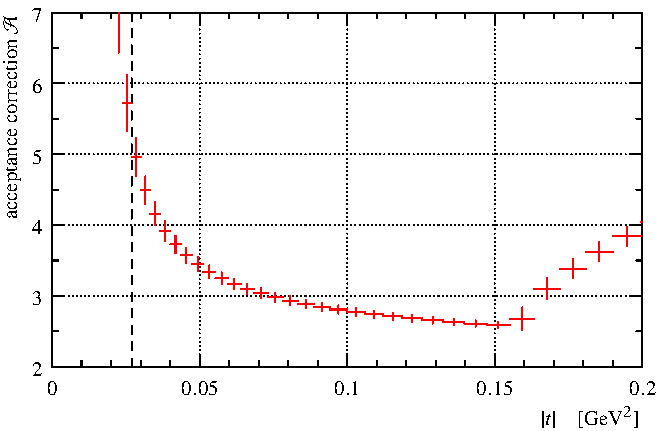
\includegraphics{fig/acc_corr_hists.pdf}
\vskip-3mm
\caption{%
\todo{caption}. DS4, 45b -- 56t, full correction, shows mean value per bin, error bar indicates standard deviation. The data left of the dashed vertical line are discarded due to excessive acceptance correction.
}
\label{fig:acceptance result}
\end{center}
\end{figure}

%-------------------------

\subsubsection{Inefficiency Corrections}
\label{sec:ineff corr}

Any inefficiency correction that does not alter the $t$-distribution shape does not need to be considered in this analysis (e.g.~the pile-up inefficiency discussed in \cite{prl111} \todo{list them all}).

The uncorrelated 1-RP inefficiency ${\cal I}_{3/4}$ is evaluated by removing a given RP from the tagging cuts, Table \ref{tab:cuts}, and calculating the fraction of recovered events. This fraction has been found to depend gently on the vertical scattering angle. The average slope of the decrease per RP is $80\un{rad^{-1}}$ with a typical uncertainty of $8\un{rad^{-1}}$. \todo{call single-RP, explain better}

The 1-RP inefficiencies are complemented by near-far correlated inefficiencies ${\cal I}_{2/4}$ from proton interactions in the near RP affecting also the far one. This contribution is determined by counting events with corresponding shower signatures and is validated with a Monte-Carlo simulation.
\todo{explain better, ask Valentina, ref to Hubert's thesis}

The full correction is calculated as
\begin{equation}
\label{efficiency}
	{\cal E}(\theta_y^*) = {1\over 1 - \left( \sum\limits_{i\in \rm RPs} {\cal I}^i_{3/4}(\theta_y^*) + 2 {\cal I}_{2/4} \right) } \ ,
\end{equation}
where the first term in parentheses typically grows from about $7$ to $10\un{\%}$ from the lowest to the highest $|\theta_y^*|$ and the second term amounts to about $3\un{\%}$.

%Trigger efficiency. Zero-bias data stream, events tagged as elastic, look at the trigger flag. NOT IN DS4 !!!
%For example for DS2, at $95\un{\%}$ CL, ${\cal I}_{\rm trig} < 8\cdot10^{-4}$. Anyway irrelevant.

\begin{figure}
\begin{center}
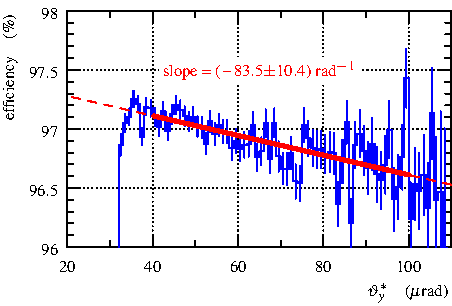
\includegraphics{fig/eff3outof4_details_fits.pdf}
\vskip-3mm
\caption{%
\todo{caption}. RP: 45, 220m, far, top. Left: drop due to acceptance, rest: ``plateau'' with slope
}
\label{fig:efficiency}
\end{center}
\end{figure}


%-------------------------

\subsubsection{Unfolding of Resolution Effects}
\label{sec:unfolding}

The correction for resolution effects has been determined by the following iterative procedure. The differential cross-section data are fitted by a smooth curve which serves as an input to a Monte-Carlo simulation using the resolution parameters determined in Section~\ref{sec:resolution}. Making a ratio between simulated histograms with and without smearing effects gives a set of per-bin correction factors. Applying them to the yet uncorrected differential cross-section yields a better estimate of the actual $t$-distribution which can be used as input to the next iteration. Due to the relatively good angular resolution, the final correction is not large: $|1 - {\cal U}| < 3\un{\%}$.

For the uncertainty estimate, the uncertainties of $\theta_x^*$ and $\theta_y^*$ resolutions (accommodating the full time variation) as well as fit-model dependence have been considered, the first contribution being dominant.

%2 iterations

\begin{figure}
\begin{center}
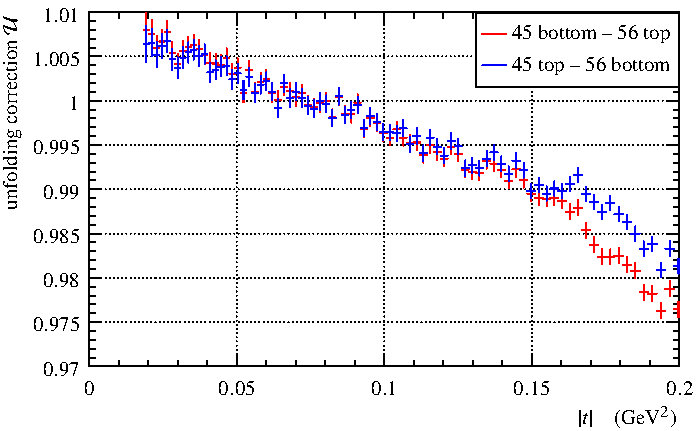
\includegraphics{fig/unfolding_correction_comparison.pdf}
\vskip-3mm
\caption{%
\todo{caption}. Points: Monte-Carlo method, solid lines: analytic calculation.
}
\label{fig:unfolding}
\end{center}
\end{figure}

%-------------------------

\subsubsection{Normalisation}
\label{sec:normalisation}

The normalisation ${\cal N}$ is determined by requiring the same cross-section integral between $|t| = 0.027$ and $0.083\un{GeV^2}$ as for dataset 1 from \cite{prl111}, where the luminosity-independent calibration was applied. The leading uncertainty of the scaling factor $4.2\un{\%}$ comes from the luminosity-independent %\linebreak 
method.

%Leading uncertainty: lumi error from DS2 ($4.2\un{\%}$), transfer to DS4 negligible (few per-mille)


%-------------------------

\subsubsection{Binning}
\label{sec:binning}

Two binnings have been considered. The ``optimised'' option sets the bin size to $1\un{\sigma}$ of the resolution in $t$. The ``per-mille'' binning is built such that each bin collects about one per-mille of the events.


%-------------------------

\subsubsection{Systematic Uncertainties}
\label{sec:systematics}

Besides the systematic uncertainties mentioned at the above analysis steps, the uncertainty of the beam momentum, $0.1\un{\%}$, needs to be considered when the scattering angles are translated into $t$, see Eq.~(\ref{eq:th t}). The systematic effects are propagated to the $t$-distribution by inserting the final cross-section into a Monte-Carlo simulation where any analysis parameter can be artificially biased.
%The results are validated with a semi-analytical calculation eventually exploiting numerical integration.
 \todo{describe procedure better}



%----------------------------------------------------------------------------------------------------

\subsection{Systematic Cross-Checks}
\label{sec:cross checks}

Compatible results have been obtained from data originating from different bunches, different diagonals and different time periods.

%----------------------------------------------------------------------------------------------------

\subsection{Final Data Merging}
\label{sec:final data merging}

Eventually, the differential cross-section histograms from both diagonals are merged. This is accomplished by a per-bin weighted average, with the weight given by inverse squared statistical uncertainty. The statistical and systematic uncertainties are propagated accordingly. For the systematic ones, the correlation between the diagonals is taken into account. For example the vertical (mis-)alignment of the RPs within one unit is almost fully correlated, thus the effect on the differential cross-section is opposite in the two diagonals, and consequently its impact is strongly reduced once the diagonals are merged.

The systematic uncertainties are summarised in Figure~\ref{fig:syst unc} where their impact on the differential cross-section is shown. The leading uncertainties include normalisation, optics imperfections and beam momentum offset. They are quantified in Table~\ref{tab:data} and can be used to approximate the covariance matrix of systematic uncertainties:
\begin{equation}
\label{eq:covar mat}
\mat V = \sum_{i=1}^{4} \vec v_i \vec v_i^{\rm T}\ ,
\end{equation}
where the $\vec v_i$'s represent the uncertainty vectors (columns) from the table.

\begin{figure*}
\begin{center}
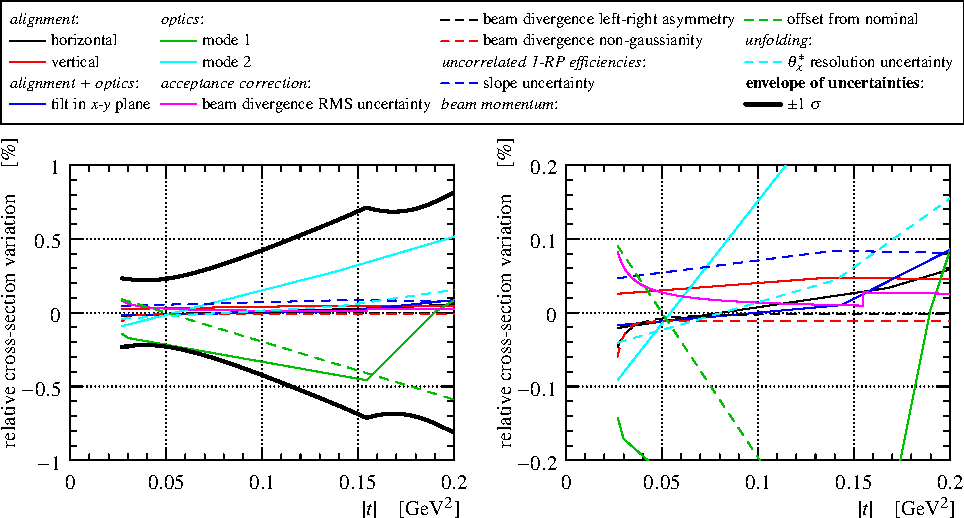
\includegraphics{fig/direct_method_mode_cmp_presentation.pdf}
\caption{%
Impact of systematic uncertainties on the differential cross-section. The two contributions due to optics correspond to the two eigenvectors of the covariance matrix of the factors scaling $\theta_x^*$ and $\theta_y^*$ (see Section~\ref{sec:optics}). \todo{explain better the two optics modes}
}
\label{fig:syst unc}
\end{center}
\end{figure*}


\begin{table*}
\caption{%
The elastic differential cross-section as determined in this analysis using the ``optimised'' binning. The three left-most columns describe the bins in $t$. The representative point gives the $t$ value suitable for fitting~\cite{lafferty94}. %uncertainty due to different fit models negligible:$10^{-7}\un{GeV^2}$
The other columns are related to the differential cross-section. The four right-most columns give the leading systematic uncertainty modes (see Section~\ref{sec:final data merging} and Figure~\ref{fig:syst unc}). \todo{explain better the 4 columns on the right}
}
\label{tab:data}
\begin{center}
\small
\setlength{\tabcolsep}{3.5pt}
\begin{tabular}{ccc@{\hskip20pt}ccccccc}
\hline
\hline
\multispan3\hss\vrule width0pt depth4pt height10pt $|t|$ bin $\unt{GeV^2}$\hss & \multispan7\hss $\d\sigma/\d t \ung{mb/GeV^2}$ \hss \cr
\multispan3\hrulefill\hbox to15pt{\hfil} & \multispan7\hrulefill \cr
left & right & representative & value & statistical     & systematic  & normalisation & optics   & optics   & beam\cr
edge & edge  & point      &       & uncertainty      & uncertainty   &       & mode 1   & mode 2   & momentum\cr
\hline
$0.02697$ & $0.03005$ & $0.02850$ & $300.94\S$ & $0.612\S$ & $12.68\S$ & $+12.66\S$ & $-0.473\S$ & $-0.259\S$ & $+0.254\S$ \cr
$0.03005$ & $0.03325$ & $0.03164$ & $284.04\S$ & $0.554\S$ & $11.91\S$ & $+11.90\S$ & $-0.495\S$ & $-0.214\S$ & $+0.204\S$ \cr
$0.03325$ & $0.03658$ & $0.03491$ & $265.59\S$ & $0.506\S$ & $11.17\S$ & $+11.15\S$ & $-0.484\S$ & $-0.172\S$ & $+0.157\S$ \cr
$0.03658$ & $0.04005$ & $0.03831$ & $247.90\S$ & $0.465\S$ & $10.44\S$ & $+10.43\S$ & $-0.472\S$ & $-0.133\S$ & $+0.114\S$ \cr
$0.04005$ & $0.04365$ & $0.04184$ & $231.95\S$ & $0.430\S$ & $\S9.740$ & $+\S9.727$ & $-0.459\S$ & $-0.0968$ & $+0.0740$ \cr
$0.04365$ & $0.04740$ & $0.04551$ & $215.35\S$ & $0.398\S$ & $\S9.061$ & $+\S9.048$ & $-0.445\S$ & $-0.0638$ & $+0.0378$ \cr
$0.04740$ & $0.05129$ & $0.04933$ & $199.89\S$ & $0.369\S$ & $\S8.405$ & $+\S8.393$ & $-0.431\S$ & $-0.0338$ & $+0.0051$ \cr
$0.05129$ & $0.05534$ & $0.05330$ & $184.55\S$ & $0.342\S$ & $\S7.775$ & $+\S7.763$ & $-0.415\S$ & $-0.0069$ & $-0.0240$ \cr
$0.05534$ & $0.05956$ & $0.05743$ & $170.71\S$ & $0.318\S$ & $\S7.171$ & $+\S7.159$ & $-0.399\S$ & $+0.0170$ & $-0.0498$ \cr
$0.05956$ & $0.06394$ & $0.06173$ & $156.62\S$ & $0.295\S$ & $\S6.594$ & $+\S6.581$ & $-0.382\S$ & $+0.0380$ & $-0.0721$ \cr
$0.06394$ & $0.06850$ & $0.06620$ & $142.96\S$ & $0.274\S$ & $\S6.044$ & $+\S6.031$ & $-0.365\S$ & $+0.0561$ & $-0.0913$ \cr
$0.06850$ & $0.07324$ & $0.07085$ & $131.31\S$ & $0.254\S$ & $\S5.521$ & $+\S5.508$ & $-0.348\S$ & $+0.0715$ & $-0.107\S$ \cr
$0.07324$ & $0.07817$ & $0.07568$ & $119.59\S$ & $0.236\S$ & $\S5.027$ & $+\S5.013$ & $-0.330\S$ & $+0.0842$ & $-0.120\S$ \cr
$0.07817$ & $0.08329$ & $0.08071$ & $108.28\S$ & $0.218\S$ & $\S4.560$ & $+\S4.546$ & $-0.312\S$ & $+0.0944$ & $-0.130\S$ \cr
$0.08329$ & $0.08862$ & $0.08593$ & $\S97.732$ & $0.202\S$ & $\S4.122$ & $+\S4.107$ & $-0.293\S$ & $+0.102\S$ & $-0.138\S$ \cr
$0.08862$ & $0.09417$ & $0.09137$ & $\S87.916$ & $0.186\S$ & $\S3.711$ & $+\S3.696$ & $-0.275\S$ & $+0.108\S$ & $-0.143\S$ \cr
$0.09417$ & $0.09994$ & $0.09702$ & $\S78.866$ & $0.172\S$ & $\S3.329$ & $+\S3.313$ & $-0.257\S$ & $+0.112\S$ & $-0.145\S$ \cr
$0.09994$ & $0.10593$ & $0.10290$ & $\S70.641$ & $0.158\S$ & $\S2.973$ & $+\S2.957$ & $-0.239\S$ & $+0.113\S$ & $-0.146\S$ \cr
$0.10593$ & $0.11217$ & $0.10902$ & $\S62.480$ & $0.145\S$ & $\S2.644$ & $+\S2.628$ & $-0.221\S$ & $+0.113\S$ & $-0.145\S$ \cr
$0.11217$ & $0.11866$ & $0.11538$ & $\S55.454$ & $0.133\S$ & $\S2.341$ & $+\S2.325$ & $-0.204\S$ & $+0.112\S$ & $-0.142\S$ \cr
$0.11866$ & $0.12540$ & $0.12199$ & $\S48.733$ & $0.122\S$ & $\S2.063$ & $+\S2.047$ & $-0.187\S$ & $+0.109\S$ & $-0.138\S$ \cr
$0.12540$ & $0.13242$ & $0.12887$ & $\S42.712$ & $0.111\S$ & $\S1.810$ & $+\S1.793$ & $-0.170\S$ & $+0.106\S$ & $-0.132\S$ \cr
$0.13242$ & $0.13972$ & $0.13602$ & $\S37.277$ & $0.102\S$ & $\S1.580$ & $+\S1.563$ & $-0.155\S$ & $+0.101\S$ & $-0.126\S$ \cr
$0.13972$ & $0.14730$ & $0.14346$ & $\S32.207$ & $0.0922$ & $\S1.372$ & $+\S1.356$ & $-0.140\S$ & $+0.0961$ & $-0.118\S$ \cr
$0.14730$ & $0.15520$ & $0.15120$ & $\S27.731$ & $0.0835$ & $\S1.185$ & $+\S1.169$ & $-0.125\S$ & $+0.0911$ & $-0.110\S$ \cr
$0.15520$ & $0.16340$ & $0.15925$ & $\S23.827$ & $0.0764$ & $\S1.016$ & $+\S1.002$ & $-0.0942$ & $+0.0855$ & $-0.102\S$ \cr
$0.16340$ & $0.17194$ & $0.16761$ & $\S20.364$ & $0.0715$ & $\S0.865$ & $+\S0.854$ & $-0.0582$ & $+0.0793$ & $-0.0938$ \cr
$0.17194$ & $0.18082$ & $0.17632$ & $\S17.249$ & $0.0666$ & $\S0.733$ & $+\S0.723$ & $-0.0298$ & $+0.0729$ & $-0.0853$ \cr
$0.18082$ & $0.19005$ & $0.18537$ & $\S14.480$ & $0.0630$ & $\S0.618$ & $+\S0.609$ & $-0.0080$ & $+0.0664$ & $-0.0769$ \cr
$0.19005$ & $0.19965$ & $0.19478$ & $\S12.124$ & $0.0585$ & $\S0.517$ & $+\S0.508$ & $+0.0052$ & $+0.0598$ & $-0.0687$ \cr
\hline
\hline
\end{tabular}
\end{center}
\end{table*}

%----------------------------------------------------------------------------------------------------

\subsection{Statistical Uncertainty Adjustment}
\label{sec:stat unc adj}
%
Examining point-to-point fluctuations in the differential cross-section using the ``optimised'' binning indicates that the statistical fluctuations have been slightly overestimated. \todo{explain the preceding argument better}
This can be alternatively demonstrated by the following procedure. The data sample is divided into several sub-samples corresponding to the same luminosity and the above-described analysis method is repeated for all of them. Then fluctuations of each bin content are determined from the several sub-samples, giving values slightly lower than the uncertainty estimates. A similar problem does not occur for the ``per-mille'' binning.
%\todo{Interpretation?}.
As a remedy, the statistical uncertainties in the ``optimised'' binning have been divided by factor $1.176$ determined by requiring the same $\chi^2$ as for the ``per-mille'' binning when a function with enough degrees of freedom is used (see the green fit in Figure~\ref{fig:data rel ob}). \todo{what function? enough dof - for what, how many? }
